\chapter{Methodology}
In this chapter, the methodology of the project will be explained in detail, covering the following aspects: dataset generation, model selection, model training, and object tracking. The dataset generation section will describe how the training data was extracted from the video and split into train and test sets. The model selection section will justify the choice of the YOLOv8 model for object detection and compare it with its size variants. The model training section will present the steps in training the YOLOv8 model on the custom dataset, including hyperparameter tuning and validation. The object tracking section will introduce the algorithm for tracking detected objects across frames. 
\newpage
\section{Dataset Generation}
The first step in this project was to generate a dataset of sperm images from the videos provided by the supervising professor. The videos were uploaded to Roboflow, a platform for data scientists for data collection and annotation. Then, the video was converted to frames using their frame extract tools, with a rate of 5 frames per second, resulting in 1400 frames. 

The next step was to label the sperms in each frame using a bounding box annotation tool. Around the first 600 images were manually labeled by drawing a rectangle around each sperm and assigning their class as a sperm. Later images were aided by a deep learning model trained by the first part of the annotation task. The model would generate a preliminary annotation on the images, and the annotators only have the task of correcting the model's predictions and labeling unnoticed sperms, reducing the workload of annotators by a significant amount. 

\begin{figure}[h]
\centering
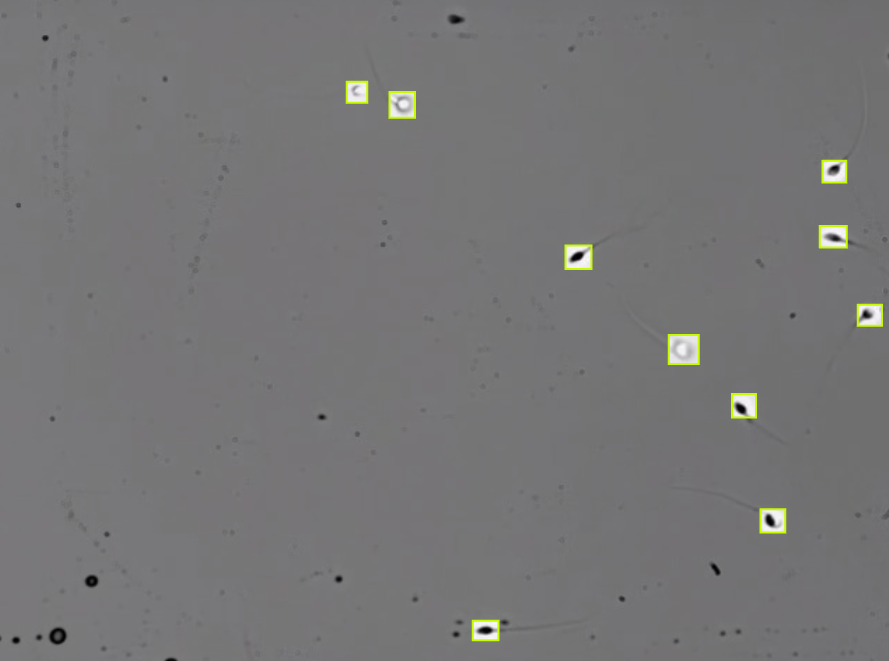
\includegraphics[width=0.85\textwidth]{Images/Labeled Frame.png}
\caption{Labeled Frame}
\end{figure}

After all 1400 images were annotated thoroughly, they underwent a full reinspection to find discrepancies in annotating rules and styles between earlier and later annotations. Although deep learning models generally can cope with such imperfections, it has been taken extra care to optimize the fitness and performance of the trained models.

\subsection{Train/Validation/Test Split}
Train/validation/test split is a technique that divides the data into three subsets: one for training the model, one for validating the model while training, and one for testing it. The training subset is used to fit the model parameters. It is crucial that the model only learns from the training set because it lowers the objective credibility of the model's performance. The validating subset measures the model's performance while training, usually after every epoch\footnote{One epoch means every image from the dataset has been fed to the training model and used to update the parameters once.} of training. The validation set gives an objective perspective of finding the optimal points to stop training from the training set to prevent the model from overfitting. Lastly, the testing subset is used to test the model with an entirely new set of data after training. Many hyperparameters can be tuned to enhance or degrade the model's performance, and test set images help compare models with different hyperparameters and find the best working setting for training. 

Although there is no golden ratio for the train/validation/test split, it is essential to set the test and validation sets to have adequate data to gain a meaningful assessment of the model. It is often misunderstood that a larger training set is always good for model performance. Still, to prevent the model from overfitting to the training set, there need to be some resources allocated to the validation and test set. For big projects with millions of training data, the testing and validation ratio can be as low as 1\%. Still, in this project, only with 1400 images, the ratio has to be significantly higher. For standard practices, according to Baheti from V7Labs, the most popular split choices for small-scale projects like this one are 60/20/20, 70/15/15, and 80/10/10. \cite{baheti} The three choices will be later examined in Subsection \ref{hyper}, as the split scheme is also part of major hyperparameters in training the model.

\subsection{Dataset Quality Analysis}
Examining the qualities of a dataset and addressing any issues is an essential process before training the model because training the model takes a lot of resources. If a dataset is poorly developed, it will affect the performance and credibility of the trained model. Usually, there are three considerations: class representations, annotation positions, and counts per frame. The first element can be neglected because this project only has one class, sperm. For the second element, Figure \ref{hitmap} is this dataset's hit map of annotations. Although there are a few hotspots, the sperms are generally well spread across the whole frame.
\newpage
\begin{figure}[ht]
\centering
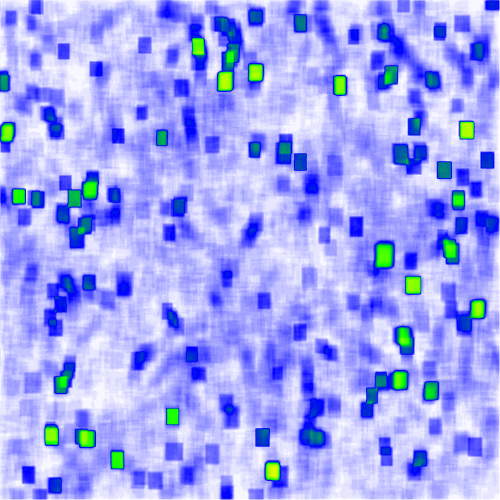
\includegraphics[width=9.6cm, height=7.2cm]{Images/hitmap.png}
\caption{Annotation Hitmap}
\label{hitmap}
\end{figure}

For the last element, Figure \ref{Hist} shows the histogram of sperm counts in all images. As most images have less than 25 sperms, the model might underperform in detecting sperms in images with more than 25 sperms. To address this issue, more images with more than 25 sperms have been allocated to the validation and test sets to find the model that works well in all environments. 

\begin{figure}[h!]
\centering
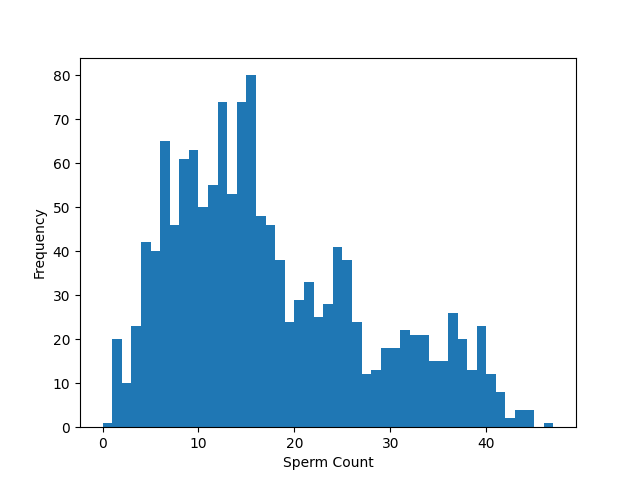
\includegraphics[width=11cm]{Images/Histogram.png}
\caption{Histogram of Sperm Counts}
\label{Hist}
\end{figure}

\subsection{Data Augmentation}
Data augmentation is a technique that can improve the performance and generalization of the trained model by increasing the size and diversity of the training data. The model learns to extract data from the image from a more diverse source of information, lowering the variance of the model. There are several data augmentation methods, but this project uses flipping, rotation, brightness, exposure, noise, and mosaic. For flipping, both horizontal and vertical flips were used, rotation was conducted within 15 degrees to both clockwise and anticlockwise, and up to 10\% brightness was added and subtracted from the images. For exposure, up to 5\% deviation was made from the original, and up to 2\% noise was added to the image. Lastly, the images were split into small parts and combined for the mosaic, which increases the model's performance in detecting small objects. The training images were tripled after data augmentation, and from some preliminary results, they have proven to increase the performance and decrease the variance of the model. 

\begin{figure}[h!]
  \begin{minipage}{\linewidth}
  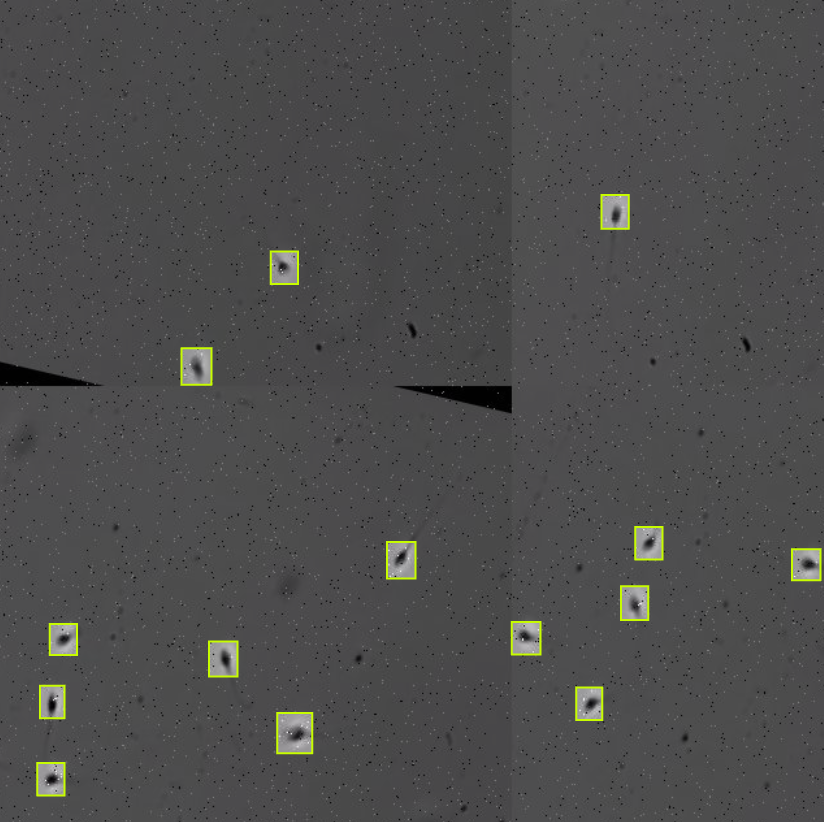
\includegraphics[width=.32\linewidth]{Images/aug1.png}\hfill
  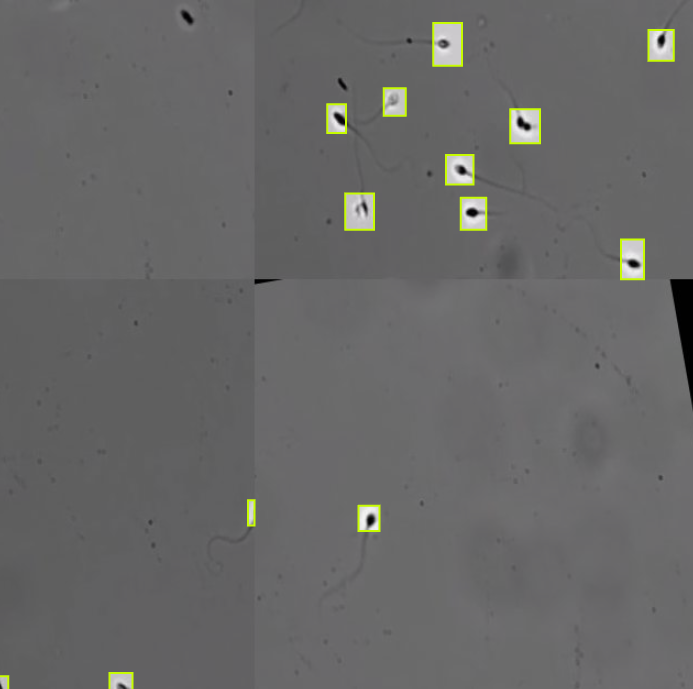
\includegraphics[width=.32\linewidth]{Images/aug2.png}\hfill
  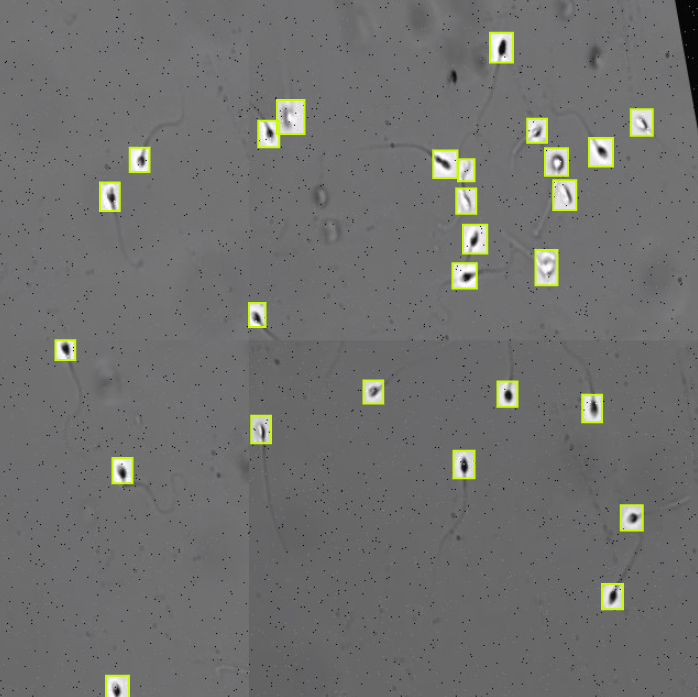
\includegraphics[width=.32\linewidth]{Images/aug3.png}%
  \end{minipage}%
  \caption{Examples of Augmented Images}
  \label{aug}
\end{figure}

\newpage
\section{Model Selection}
Model selection is an essential step in the methodology of any machine learning project, as it determines the accuracy and validity of the results. As described in Chapter \ref{lit}, YOLO models are the most popular models for object detection, and even in sperm detection tasks, many researchers have proven their effectiveness in detecting sperm cells. As many variant models exist in YOLO, it is very important to find which one to use. From the general understanding of the data science community, YOLOv5 and YOLOv8 are considered the most effective models, with excellent community support and user-friendly resources. As shown in Figure \ref{yolocomp}, because YOLOv8 had better performance at a similar latency rate, the project chose YOLOv8 for the detection model.

\subsection{Model Size}
YOLOv8 provides 5 model sizes: nano, small, medium, large, and x-large. Bigger models have more parameters and higher performance, but smaller models take a shorter time to train and have smaller latencies. Because there were insufficient computational resources, this project only tested three smaller models. Each model was trained for 25 epochs with the same training conditions, and the result is shown in Table \ref{yolotable}.

\begin{table}[ht]
\centering
\begin{tabular}{|l|c|c|c|c|c|}
\hline
Size   & mAP50 & mAP50-95 & \begin{tabular}[c]{@{}c@{}}Training Time\\ (seconds/epoch)\end{tabular} & \begin{tabular}[c]{@{}c@{}}Latency\\ (ms/frame)\end{tabular} & \begin{tabular}[c]{@{}c@{}}Model Size\\ (MB)\end{tabular} \\ \hline
Nano   & 0.960 & 0.515    & 105                                                                     & 10                                                           & 6.0                                                       \\ \hline
Small  & 0.972 & 0.531    & 115                                                                     & 21                                                           & 23.3                                                      \\ \hline
Medium & 0.976 & 0.584    & 125                                                                     & 38                                                           & 197.9                                                     \\ \hline
\end{tabular}
\caption{Comparison of YOLOv8 Models}Training GPU: Tesla T4, Latency GPU: GTX 1660 Super
\label{yolotable}
\end{table}

For the accuracy of the models, a specific standard for object detection tasks was used. mAP stands for mean average precision, and for mAP50, the intersection over union (IOU) threshold was 50\%. The nano model has a performance of about 96\% of the detections made by the model had 50\% or more IOU with the ground truth. The IOUs of detections are calculated in Figure \ref{iou}. mAP50-95 is the weighted average for all mAPs over 50\% to 95\%.

\newpage

\begin{figure}[ht]
\centering
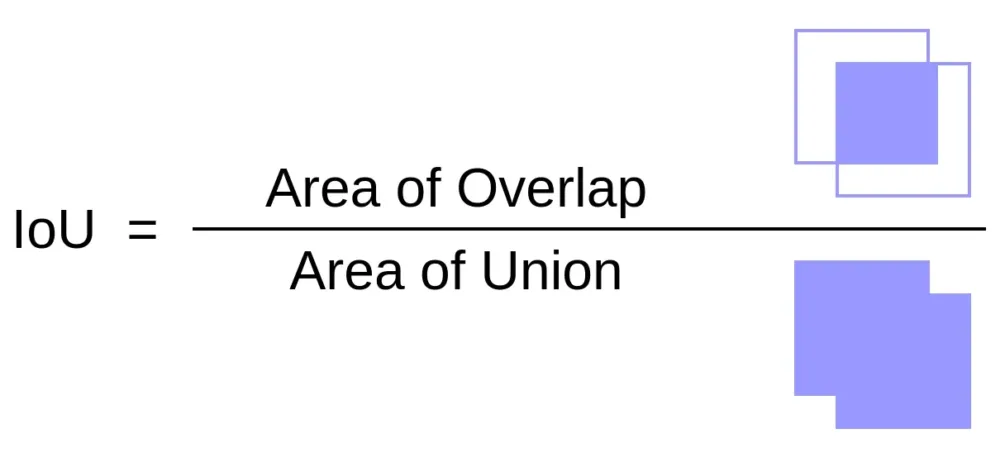
\includegraphics[width=13cm]{Images/iou.png}
\caption{IOU Calculation Method \cite{iou}}
\label{iou}
\end{figure}

From Table\ref{yolotable}, it can be seen that even the nano-sized model is performing well. However, it is still noticeable that the gap between nano and small models is quite large. Although the medium-sized model performed the best, the latency measured with the provided GPU was still too high to be used in a real-time tracking model. Therefore, the small-sized model was chosen to be used in this project. 

\newpage
\section{Model Training}
This section will explain how the model was trained. The model training process consists of three main steps: environment setup, hyperparameter tuning, and validation. The hardware and software requirements and the libraries and frameworks used for implementing the model will be explained in the environment setup step. In the hyperparameter tuning step, the methods and criteria for selecting the optimal values of the model parameters, such as learning rate, batch size, number of epochs, etc., will be discussed. The validation step will discuss how the models are tested with a held-out test set and validated.

\subsection{Environment Setup}
Like many machine learning projects, Python language was used in this project. To download and install YOLOv8, one can use Python's built-in package installer, pip. Several other libraries need to be installed together, which will be automatically detected by the installer and installed together. 
\begin{verbatim}
    pip3 install ultralytics
\end{verbatim}
The above line should be run at the Command Prompt. It is always better to download and install libraries in a virtual environment to prevent collisions. The above line should install almost all packages and libraries for this project. Still, for the remaining packages, if any, one can find \verb|requirements.txt| at \href{https://github.com/rladntjr7/FYP}{\underline{GitHub}} and run the following line at Command Prompt.
\begin{verbatim}
    pip3 install -r requirements.txt
\end{verbatim}

GPU support comes in handy for training and predicting with machine learning models. GPU parallel computing is a lot faster than CPU. Depending on the model, the GPU is 20 \~{} 100 times faster than the CPU. For training, Google Colab, a Cloud GPU provider, was used. GTX 1660 super was used as this project's primary computation unit for any other applications. Moreover, the CUDA framework from NVIDIA also needs to be installed for GPU involvement in model training. 
\newpage
\subsection{Hyperparameter Tuning}\label{hyper}
Many hyperparameters can be tuned to increase the model performance. Finding the optimal setup includes a lot of guesswork, and every project needs a different setup, so it is challenging to refer to others' work. However, there is a general guideline in the machine learning community written by AI engineers from Google, and it is called Deep Learning Tuning Playbook. \cite{tuningplaybookgithub} 

From the playbook, some important prerequisites need to be set before tuning the model:
\begin{itemize}
    \item Dataset is well organized.
    \item The environment is well prepared to minimize the time spent on the execution of training and validation of the model.
    \item The metric for analyzing the performance of the model is selected.
\end{itemize}

From the works from the previous sections, the first two items are already assessed. The main criteria for assessing the model will be mAP50, as the model does not require a very high precision due to the presence of the Kalman filter in the tracking stage. 

To increase the training throughput, a larger batch size\footnote{Batch size governs the number of training samples the model trains before updating the model's parameters. A larger batch size is advantageous because it decreases the number of steps within an epoch.} was used to expedite the training process. A higher training throughput will lead to a faster optimization of the model. The ideal batch size is usually the biggest size that the hardware can handle. From some experiments, the largest batch size available from Google Colab's Tesla T4 GPU is 42, and it decreased the training time by 30 seconds per epoch for the small-sized model. To further increase the speed, A100 GPU was used from the premium version of Google Colab, and it decreased the training time to around 15 seconds per epoch by using a batch size of 142. 

Some of the first things to consider were the dataset split and optimizer. As introduced earlier in this report, three splits will be tested, 60/20/20, 70/15/15, and 80/10/10. Four optimizers are available with YOLOv8: SGD, Adam, AdamW, and RMSProp. First, the data split will be tested by training the model for 20 epochs for each split. The result is displayed in Table \ref{splittable}.

\newpage

\begin{table}[h]
\centering
\begin{adjustbox}{max width=\textwidth}
\begin{tabular}{|c|cc|cc|cc|cc|}
\hline
\multirow{2}{*}{\textbf{Split}} & \multicolumn{2}{c|}{\textbf{Trial 1}}                                                                                                        & \multicolumn{2}{c|}{\textbf{Trial 2}}                                                                                                        & \multicolumn{2}{c|}{\textbf{Trial 3}}                                                                                                        & \multicolumn{2}{c|}{\textbf{Average}}                                                                                                        \\ \cline{2-9} 
                                & \multicolumn{1}{c|}{\begin{tabular}[c]{@{}c@{}}Validation\\ Accuracy\end{tabular}} & \begin{tabular}[c]{@{}c@{}}Test\\ Accuracy\end{tabular} & \multicolumn{1}{c|}{\begin{tabular}[c]{@{}c@{}}Validation\\ Accuracy\end{tabular}} & \begin{tabular}[c]{@{}c@{}}Test\\ Accuracy\end{tabular} & \multicolumn{1}{c|}{\begin{tabular}[c]{@{}c@{}}Validation\\ Accuracy\end{tabular}} & \begin{tabular}[c]{@{}c@{}}Test\\ Accuracy\end{tabular} & \multicolumn{1}{c|}{\begin{tabular}[c]{@{}c@{}}Validation\\ Accuracy\end{tabular}} & \begin{tabular}[c]{@{}c@{}}Test\\ Accuracy\end{tabular} \\ \hline
60/20/20                        & \multicolumn{1}{c|}{96.8\%}                                                        & 96.2\%                                                  & \multicolumn{1}{c|}{96.4\%}                                                        & 95.6\%                                                  & \multicolumn{1}{c|}{96.8\%}                                                        & 96.2\%                                                  & \multicolumn{1}{c|}{96.7\%}                                                        & 96.0\%                                                  \\ \hline
70/15/15                        & \multicolumn{1}{c|}{97.6\%}                                                        & 95.1\%                                                  & \multicolumn{1}{c|}{97.6\%}                                                        & 95.1\%                                                  & \multicolumn{1}{c|}{97.6\%}                                                        & 94.0\%                                                  & \multicolumn{1}{c|}{97.6\%}                                                        & 94.7\%                                                  \\ \hline
80/10/10                        & \multicolumn{1}{c|}{97.9\%}                                                        & 95.9\%                                                  & \multicolumn{1}{c|}{97.7\%}                                                        & 95.4\%                                                  & \multicolumn{1}{c|}{97.7\%}                                                        & 95.4\%                                                  & \multicolumn{1}{c|}{97.8\%}                                                        & 95.6\%                                                  \\ \hline
\end{tabular}
\end{adjustbox}
\caption{Comparison of Different Dataset Split}Metric: mAP50
\label{splittable}
\end{table}

In Table \ref{splittable}, three trials were conducted for each split, and the average accuracies were shown in the last two columns. Of all splits, the 70/15/15 split performed the worst. Presumably, the 60/20/20 split benefitted the model with the testing performance from the larger validation set, and the 80/10/10 split had a greater fit to the data with the larger training set. 

Although the 80/10/10 split performed the best in validation, its testing accuracy was lower than 60/20/20. Because testing accuracy is the most important criterion and with the lowest variance, the 60/20/20 split was selected for this project. 

The next step is choosing the optimizer. From the above four options, SGD\footnote{Stochastic Gradient Descent} is the most basic option, where the parameters are updated from a few random samples from the batch. SGD is fast because the model does not have to learn from all training samples within the batch. However, because optimization is a global minimum problem in a multi-dimensional space, SGD's inability to escape from local minima quickly is a critical disadvantage. The other three optimizers try to mitigate this issue using different techniques. RMSProp uses the moving average of gradients and reduces the oscillation of weights by dividing the moving averaged gradient by the gradient's root mean square (RMS). On the other hand, Adam combines RMSProp with the concept of momentum, where the gradient is less likely to be reduced when the history of gradients has a similar direction. AdamW involves weight decay, increasing the convergence rate and the generalization of the model. 

For many cases, AdamW is the optimal choice, and many indicate that using AdamW is not degrading the model's performance in most cases while reducing overfitting.\cite{adamw} Therefore, AdamW will be the main optimizer for training in this project. Other optimizers will be assessed as well if AdamW underperforms significantly. 
\newpage
The learning rate has to be scheduled for the last step before training the model. Learning rates are significant in training because if the rate is too low, the model will not gain any updates from the training. If the rate is too high, the gradients will make the model oscillate, making it harder to reach the global minimum or even diverge. 

This project uses the pre-trained model by the makers of YOLOv8. The original model was trained from the COCO dataset. \cite{coco} Because the weights in earlier layers are already optimized to find specific characteristics from the images, the learning rate has to be kept low. Three learning rates will be tested to find the optimal training setting, which will be 0.001 as the original setting, 0.0005, and 0.0001. Figure \ref{lrcomp} shows the effect of different learning rates on the training loss.

\begin{figure}[h]
    \centering
    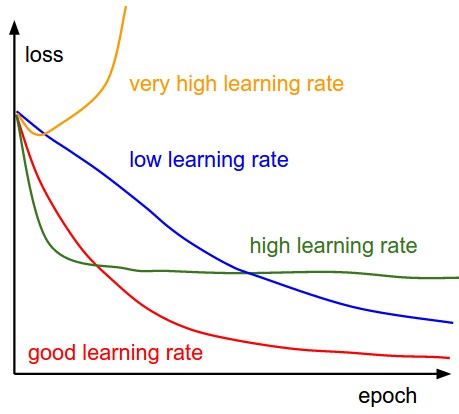
\includegraphics[width = .8\textwidth]{Images/learning rate.jpeg}
    \caption{Learning Rate Comparison \cite{cs231n}}
    \label{lrcomp}
\end{figure}

\newpage
The three learning rates were tested with 50 epochs each, and Figure \ref{lrtest} shows the effect of the learning rate on training losses. 

\begin{figure}[h]
  \begin{minipage}{\linewidth}
  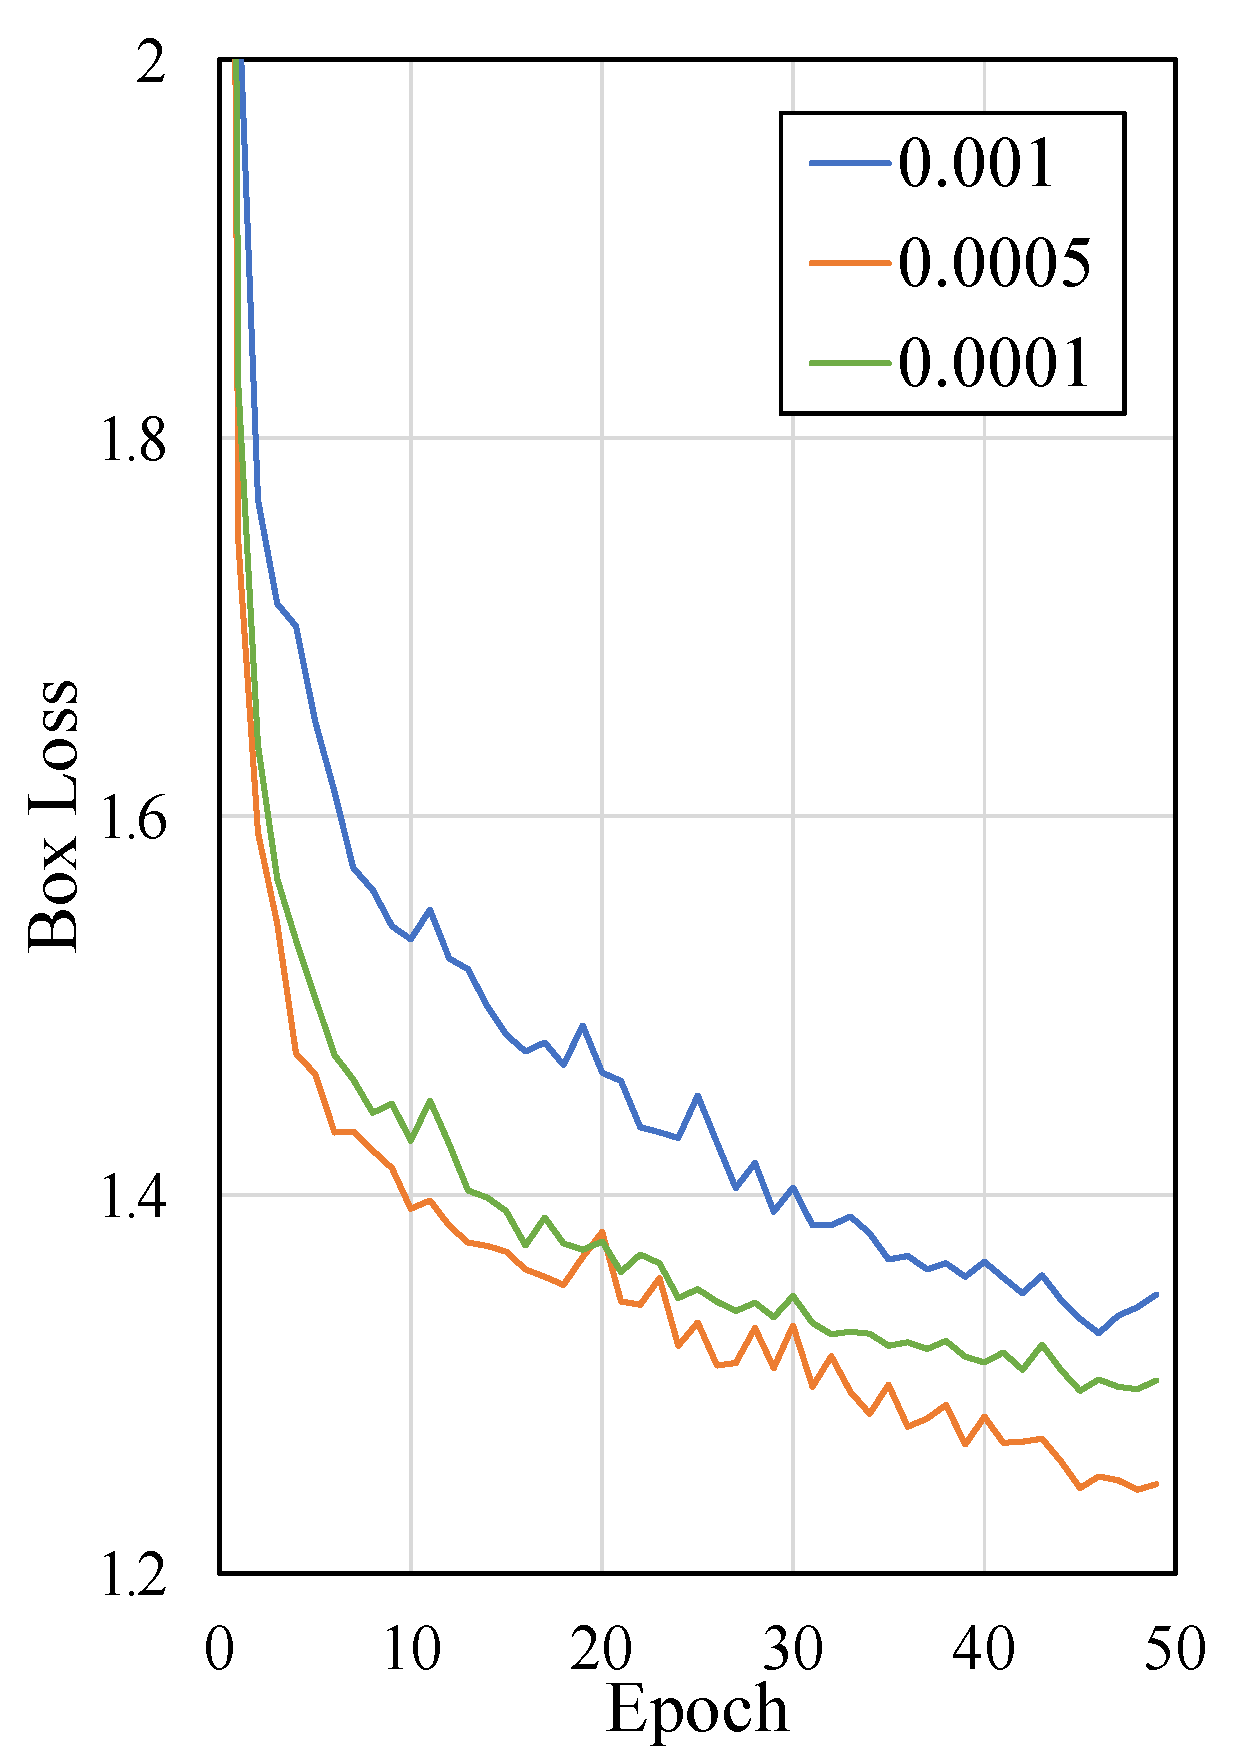
\includegraphics[width=0.33\linewidth]{Images/box loss.pdf}\hfill
  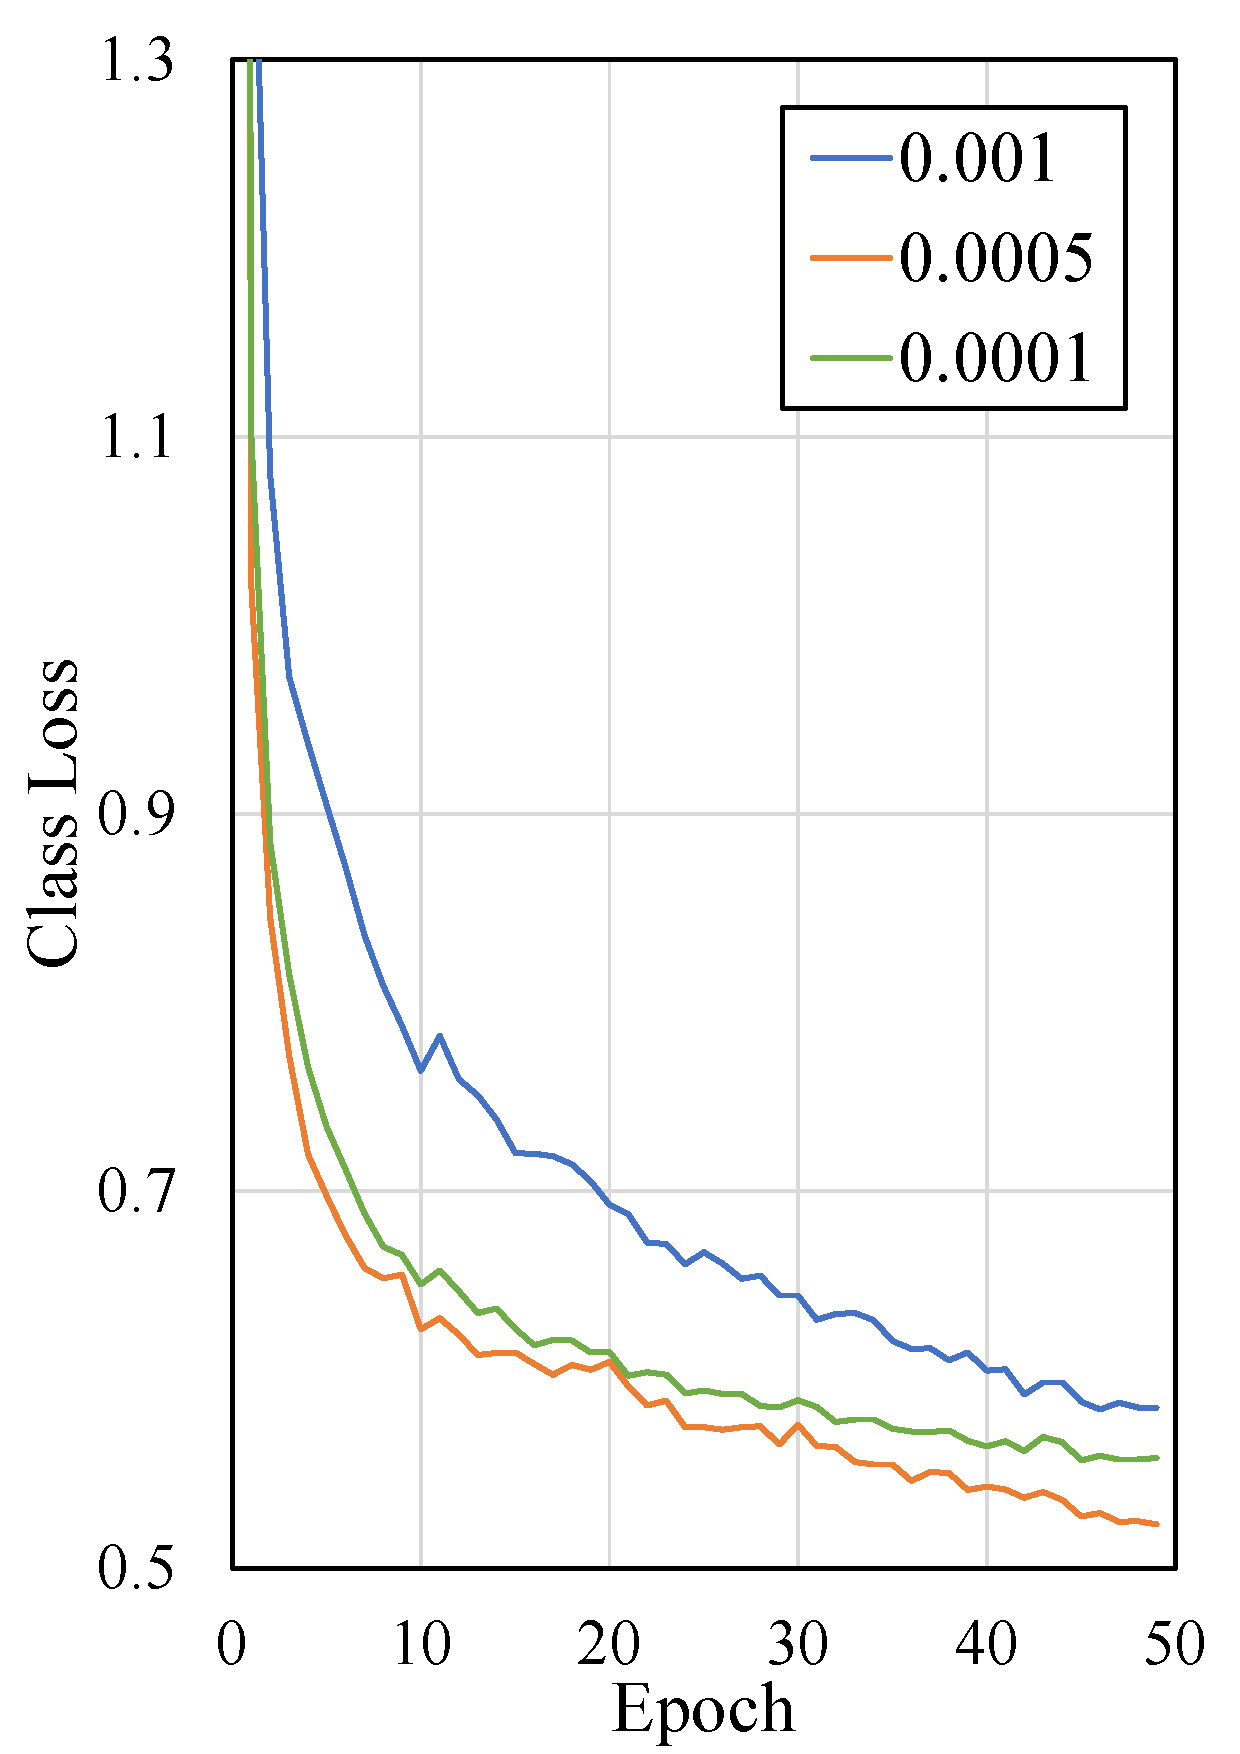
\includegraphics[width=0.33\linewidth]{Images/class loss.pdf}\hfill
  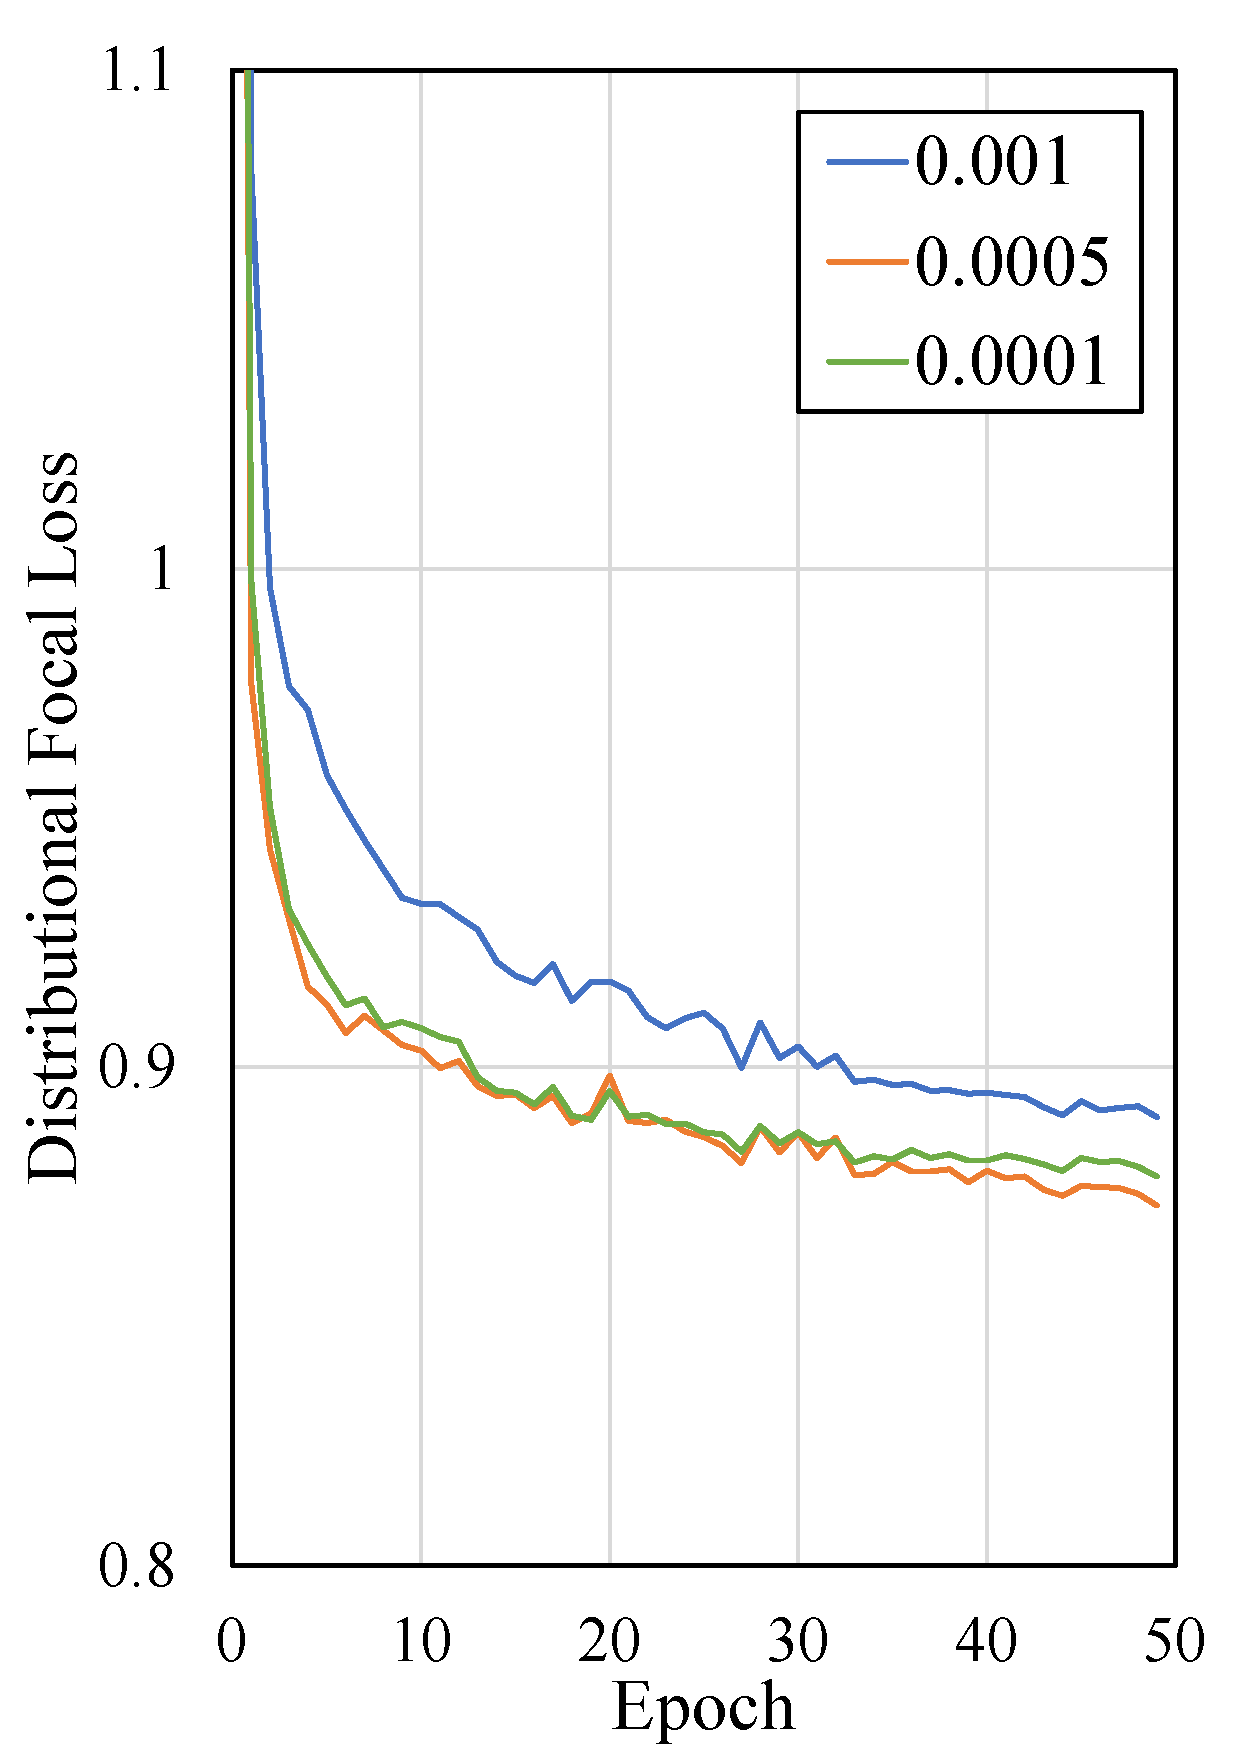
\includegraphics[width=0.33\linewidth]{Images/dfl loss.pdf}%
  \end{minipage}%
  \caption{Learning Rate Test Result}
  \label{lrtest}
\end{figure}

When the results are compared with Figure \ref{lrcomp}, the 0.001 learning rate seems to be too high, and the 0.0001 rate is too low. It can be found that the learning rate of 0.0005 is the adequate learning rate for this project. Although 54 hyperparameters can be tuned for the training of a YOLOv8 model, most of them are already optimized for general training and are not as important as the ones tuned explicitly in this project. Moreover, due to the limitation of computational resources, hyperparameter tuning will be finalized at this stage. 

\subsection{Validation}
Model validation evaluates the model's performance if it has reached the target and can be used for the intended purpose. Model validation is an essential step in any machine learning project. It helps ensure that the model is not overfitting or underfitting to the data and generalizing well to unseen scenarios. After training the model with finalized settings for 100 epochs, the model will be evaluated in Chapter \ref{results}, using various metrics and plots, such as accuracy, precision, recall, F1-score, etc.

\newpage
\section{Object Tracking}
This section will explain what methods were used in the tracking part of the project. Object tracking of sperm cells is difficult because they do not always move consistently, often becoming out of focus and undetected by the model. This project managed to keep track of most sperms in the frames, and the primary method is shown as the flow chart in Figure \ref{flowchart}.

To facilitate the tracking of sperm, a sperm class was made under \verb|sperm.py|, where the sperm needs an identification number and the coordinates of the bounding box for declaration. The class's \verb|__init__| function assigns various attribute elements for tracking, including many matrices for the Kalman filter and activity indexes. Detailed analysis of the tracking algorithm will be described in the following subsections. 

\clearpage
\begin{figure}[ht!]
\centering
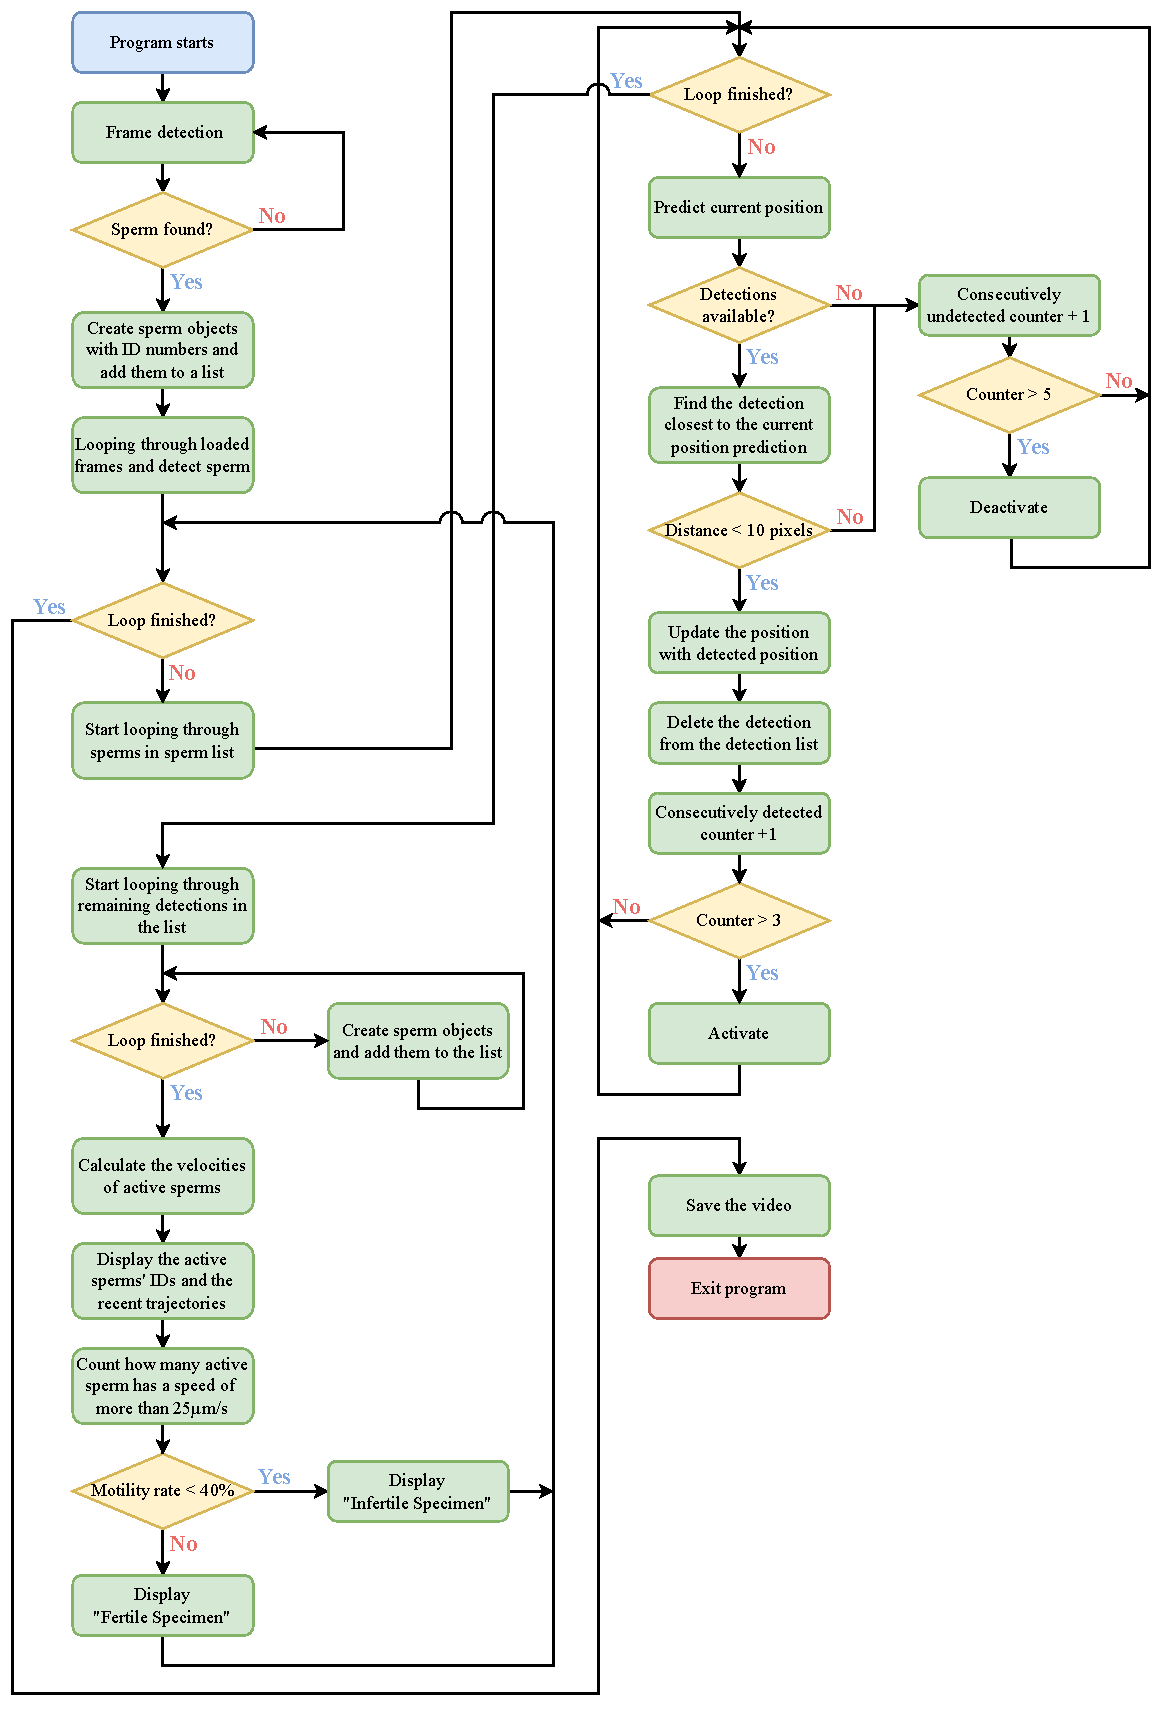
\includegraphics[width=13cm]{Images/flowchart.drawio.pdf}
\caption{Flowchart of the Program}
\label{flowchart}
\end{figure}


\subsection{Kalman Filter} \label{kalman}
Kalman filters, usually called noise filters, find optimal state estimations based on uncertain measurements and predictions. \cite{kalman}\cite{kalman2} Kalman filters are used anywhere an accurate status estimation is needed, including GPS, Radar, economics, etc. Object tracking systems also require optimal estimations to track the objects smoothly, even if they are occluded or blurry. Kalman filter is especially very useful in this project because, from its recursive nature, the Kalman filter only uses a minimal amount of memory, which is very useful when sometimes there are hundreds of items to track throughout the whole video. 

The basic equations of the Kalman filters are Equations \ref{kal1} and \ref{kal2}. 
\begin{equation} \label{kal1}
    X_k = AX_{k-1} + Bu_{k-1}+w_{k-1}
\end{equation}
\begin{equation} \label{kal2}
    Z_k = HX_k + v_k
\end{equation}
where Equation \ref{kal1} is the prediction equation of the Kalman filter from the previous information about an object. Equation \ref{kal2} represents the current measured status. \(w_k\) and \(v_k\) represent the noises from the prediction and measurement, and they are assumed to be following the Gaussian distribution with covariance matrices \(Q\) and \(R\), respectively.

The following kinematic equations were set up to derive the components for Equation \ref{kal1}.
\begin{equation} \label{xcoor}
x_k=x_{k-1}+\Dot{x}_{k-1}\Delta t + \frac{1}{2}\Ddot{x}_{k-1}\Delta t ^2
\end{equation}
\begin{equation} \label{xvel}
\Dot{x}_k=\Dot{x}_{k-1}+\Ddot{x}_{k-1}\Delta t
\end{equation}

Equations \ref{xcoor} and \ref{xvel} can be simplified to a single matrix, 
\begin{equation} \label{xmat}
X_k = \begin{bmatrix} x_k \\ \Dot{x}_k\end{bmatrix}=\begin{bmatrix}
    x_{k-1}+\Dot{x}_{k-1}\Delta t + \frac{1}{2}\Ddot{x}_{k-1}\Delta t ^2 \\
    \Dot{x}_{k-1}+\Ddot{x}_{k-1}\Delta t
\end{bmatrix}
\end{equation}

Equation \ref{xmat} can be further simplified to matrix multiplication,
\begin{equation} \label{xmatsimp}
X_k = \begin{bmatrix} x_k \\ \Dot{x}_k\end{bmatrix} = \begin{bmatrix}
    1 & \Delta t \\
    0 & 1
\end{bmatrix}
X_{k-1}
+
\begin{bmatrix}
    \frac{\Delta t^2}{2} \\
    \Delta t
\end{bmatrix}
\Ddot{x}_{k-1}
\end{equation}

For the two-dimensional version of Equation \ref{xmatsimp},
\begin{equation} \label{xymat}
X_k = 
\begin{bmatrix} 
x_k \\ 
y_k \\ 
\Dot{x}_k \\ 
\Dot{y}_k
\end{bmatrix} 
= 
\begin{bmatrix}
    1 & 0 & \Delta t & 0 \\
    0 & 1 & 0 & \Delta t \\
    0 & 0 & 1 & 0 \\
    0 & 0 & 0 & 1
\end{bmatrix}
X_{k-1}
+
\begin{bmatrix}
    \frac{\Delta t^2}{2} & 0 \\
    0 & \frac{\Delta t^2}{2} \\
    \Delta t & 0 \\
    0 & \Delta t
\end{bmatrix}
\alpha _{k-1}
\end{equation}
where \(\alpha_{k}\) is a matrix of accelerations at time \(k\).

The two matrices of Equation \ref{xymat} are \(A\) and \(B\) from Equation \ref{kal1}.
\begin{equation}
    A = \begin{bmatrix}
        1 & 0 & \Delta t & 0 \\
        0 & 1 & 0 & \Delta t \\
        0 & 0 & 1 & 0 \\
        0 & 0 & 0 & 1
    \end{bmatrix}
    B = \begin{bmatrix}
        \frac{\Delta t^2}{2} & 0 \\
        0 & \frac{\Delta t^2}{2} \\
        \Delta t & 0 \\
        0 & \Delta t
    \end{bmatrix}
\end{equation}

The process noise covariance matrix \(Q\) can be defined as follows:
\begin{equation} \label{covQ}
Q = 
\begin{bmatrix}
    \sigma ^2_x & 0 & \sigma_x \sigma_{\Dot{x}} & 0 \\
    0 & \sigma ^2_y & 0 & \sigma_y \sigma_{\Dot{y}} \\
    \sigma_x \sigma_{\Dot{x}} & 0 & \sigma ^2_{\Dot{x}} & 0 \\
    0 & \sigma_y \sigma_{\Dot{y}} & 0 & \sigma ^2_{\Dot{y}}
\end{bmatrix}
\end{equation}
where it is assumed that there is no correlation between the two axes. 
The equation can be further simplified when the standard deviations of position and velocities are assumed to be \(\frac{\Delta t^2}{2}\sigma_a\) and \(\Delta t \sigma_a\), respectively, where \(\sigma_a\) is the standard deviation of the acceleration, and \(\Delta t\) is the time between timesteps. 

The process noise covariance matrix is now simplified as follows:
\begin{equation} \label{covQsimp}
Q = 
\begin{bmatrix}
    \frac{\Delta t^4}{4} & 0 & \frac{\Delta t^3}{2} & 0 \\
    0 & \frac{\Delta t^4}{4} & 0 & \frac{\Delta t^3}{2} \\
    \frac{\Delta t^3}{2} & 0 & \Delta t^2 & 0 \\
    0 & \frac{\Delta t^3}{2} & 0 & \Delta t^2
\end{bmatrix}
\sigma_a^2
\end{equation}

The transformation matrix \(H\) from Equation \ref{kal2} is defined as:
\begin{equation} \label{transmat}
H = 
\begin{bmatrix}
    1 & 0 & 0 & 0 \\
    0 & 1 & 0 & 0
\end{bmatrix}
\end{equation}
In this project, only the positions are measured by the detection model. Therefore, the velocity components are neglected. 

The measurement noise covariance matrix is defined as:
\begin{equation} \label{noiscov}
R = 
\begin{bmatrix}
\sigma_x^2 & 0 \\
0 & \sigma_y^2
\end{bmatrix}
\end{equation}
where the detection model is assumed that there are no dependencies between two coordinates during detections.

Moreover, it can also be assumed that the standard deviations of both coordinates are similar to each other, and the Equation \ref{noiscov} can be simplified as:
\begin{equation}
    \label{noiscovsimp}
    R=
    \begin{bmatrix}
        \sigma_m^2 & 0 \\
        0 & \sigma_m^2
    \end{bmatrix}
\end{equation}
where \(\sigma_m^2\) is the standard deviation of measurement in both axis. 

\subsubsection{Prediction}
A priori state (before status is updated with the measurement) is estimated with the following equation to predict the current status based on previous information.
\begin{equation}
    \label{priori}
    \hat{X}_k^- = A\hat{X}_{k-1} + B u_{k-1}
\end{equation}
where \(\hat{X}_k^-\) is the priori state estimate, and \(\hat{X}_{k-1}\) is the posteriori state estimate (after update with the measurement) from the last timestep \(k-1\). 

The priori error covariance matrix is calculated as follows:
\begin{equation}
    \label{prioricov}
    P^-_k = AP_{k-1}A^T + Q
\end{equation}
where \(P^-_k\) is the priori error covariance matrix, and \(P_{k-1}\) is the posteriori error covariance matrix from the last timestep.

\subsubsection{Update}
As the first step of the update stage, the Kalman gain \(K_k\) is calculated as the following equation.
\begin{equation}
    K_k=P^-_k H^T (HP^-_kH^T+R)^{-1}
\end{equation}
To update the prior state estimate to the posteriori state estimate, it has to be added by the product of the Kalman gain \(K_k\) and the measurement residual. The measurement residual is the difference between the current measurement and the previous estimation. Therefore it is \(Z_k - H\hat{x}^-_k\). So, the posteriori state estimate is calculated as follows: 
\begin{equation}
    \hat{X}_k = \hat{X}_k^- + K_k(Z_k - H\hat{x}^-_k)
\end{equation}

Also, the error covariance matrix \(P_k\) is updated, which will be used in the next timestep. 
\begin{equation}
    P_k = (I-K_h H)P^-_k
\end{equation}

\subsection{Tracking Algorithm}
This subsection will explain the tracking algorithm of this program in detail, including the utilization of the Kalman filter as defined in Subsection \ref{kalman}.

When the program starts, it brings the video and the detection model. The first frame is detected, and each detection is given an identification number and stored inside the \verb|sperm_list|. If there is no sperm in the first frame, the program loops until there is any sperm found. When the sperm is declared, all the Kalman filter components are initialized with the input parameters. 

Afterward, the program loops through the following frames in the video. For each frame, the program loops through the sperms in the \verb|sperm_list| and predicts the priori estimates with the \verb|predict()| function. For each sperm, it is checked if any detections are available in the detection list, and if there are, the distance between the closest detection and priori estimate is calculated. If it is less than 10 pixels, the posteriori estimate is calculated using the \verb|update(detected coordinates)| function, and the detection is removed from the list. The sperm needs to be detected in 3 frames consecutively to become active status. 

If the sperm does not have any available detection because all were taken by the previous sperms in the \verb|sperm_list| or the distance between the detection and the priori estimate was more than 10 pixels, the consecutive undetected counter increases, and if the counter reaches more than 5, the sperm is now deactivated. 

When all sperms in the \verb|sperm_lsit| are assessed, the remaining detections are declared sperm and added to the \verb|sperm_list|. They also get identification numbers, and all components for the Kalman filter are initialized.

For all sperms, based on the past 60 frames, the velocities are calculated. The ID number and trajectories are displayed in the frame next to the sperms. If there are more than 40\% of total active sperms that have a speed of 25\(\mu m/s\), the "Fertile Specimen" message is displayed. Otherwise, "Infertile Specimen" is displayed. 

After addressing all sperms and new detections, the program moves to another frame. The time between each frame is recorded and displayed as the FPS. When the video ends, the video is saved at a designated location. Lastly, the program is exited. 